\subsection{Página inicial}

Esta página é dirigida a todos os utilizadores e visitantes do sistema, é a primeira página e não é necessário ter um registo no sistema para a consultar.

Nesta página pretende-se demonstrar todas as funcionalidades do sistema, cativar novos utilizadores e promover a aplicação.\\

No inicio da página optou-se por colocar um \textit{slider} que de uma forma simples e sucinta explicita as principais vantagens do sistema como ser acessível em qualquer dispositivo e principais vantagens para os alunos e para os docentes.

De seguida são listados os diferentes tipos de utilizadores para os quais o sistema oferece vantagens, e uma frase que pretende cativar esse grupo de utilizadores a utilizar o sistema.

Como os estudantes constituem a maior parte dos potenciais utilizadores do sistema, decidiu-se listar as principais categorias onde estes utilizadores vão obter mais vantagens ao utilizar a aplicação.

Depois de frases de incentivo ao registo e imagens demonstrativas, são listadas as categorias onde os docentes vão obter mais vantagens ao utilizar a aplicação.\\

Nesta página os utilizadores não registados, para além de consultar as funcionalidades do sistema, podem aceder ao mapa do site, sobre nós, pesquisar por projetos públicos e entrar ou registar no sistema.
Os utilizadores registados para além das possibilidades referidas, podem aceder a um painel de gestão de projetos e unidades curriculares.\\ 

Na Figura~\ref{fig:home_page} pode ser consultada uma imagem demonstrativa da página desenvolvida.

\begin{figure}[H]
  \centering
  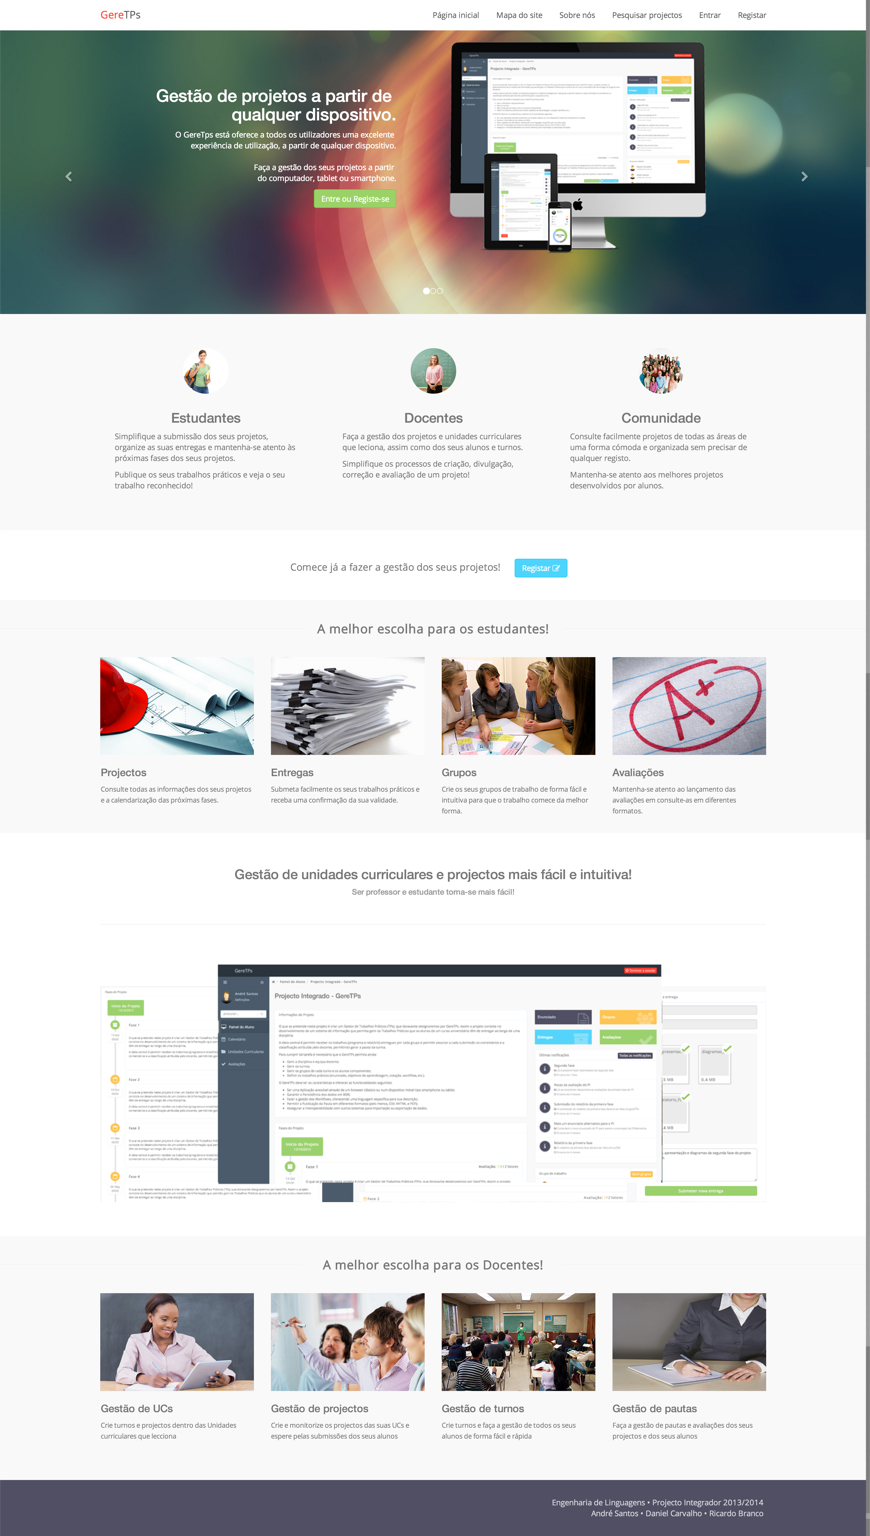
\includegraphics[width=.7\textwidth,center]{images/implementacao/home_page}
  \caption{Página inicial}
  \label{fig:home_page}
\end{figure}
